\documentclass{article}
\usepackage[utf8]{inputenc}
\usepackage[spanish]{babel}
\usepackage{natbib}
\usepackage{graphicx}
\usepackage{mathtools}
\usepackage{color}
\usepackage{float}
\usepackage{fancyhdr}
\usepackage{adjustbox}
\usepackage{verbatim}


\pagestyle{fancy}
\lhead{Grupo 4 - Turno 7}
\chead{Trabajo Practico Nro 5}
\rhead{Primer Cuatrimestre 2015}

\begin{document}
\section{Introducción Teórica}
Un alambre que transporta una corriente y que se encuentra inmerso en un campo magnético, experimenta una fuerza que es usualmente llamada fuerza magnética. La magnitud y dirección de esta fuerza depende de cuatro variables:
\begin{itemize}
  \item la longitud del alambre L
  \item la intensidad del vector inducción magnética $\overrightarrow{B}$
  \item la magnitud de la corriente I
  \item el ángulo entre el alambre y el campo $/theta$
\end{itemize}
Esta fuerza magnética puede ser descripta matemáticamente como: 
\begin{equation}
\overrightarrow{F}=q (v\times \overrightarrow{B}) = I \overrightarrow{L}\times\overrightarrow{B} 
\end{equation}

\section{Objetivos}
En esta experiencia se comprobará la validez de la ecuación (1). Para ello se variarán de a
uno los parámetros que intervienen en la expresión de la fuerza producida por un campo
magnético externo uniforme y constante sobre un alambre que transporta corriente: la intensidad de
la corriente y longitud del alambre. Para cada caso se graficará y comprobará la relación lineal entre las distintas magnitudes. Se utilizará como
método de aproximación lineal el de cuadrados mínimos. 

\section{Materiales}
Se dispone de varias plaquetas que
tienen incorporados distintos circuitos cuya longitud varía y se midió en la experiencia, una balanza cuya mínima división es de 10 mg, imanes y un montaje para las plaquetas.

\section{Desarrollo}
\subsection{Fuerza en función de la corriente}
Para esta primera experiencia:

\begin{enumerate}
  \item Se armó el dispositivo con uno de los circuitos.
  \item Se determinó la masa del porta imán y de los imanes sin corriente.
  \item Se varió la corriente en pasos de 0,5A hasta 3A y se determinó la nueva "masa" del sistema.
  \item Se calculó la fuerza magnética.
  \item Se graficaron los resultados.
  \item Se obtuvo el campo el valor para el campo magnético B producido por el imán.
\end{enumerate}

\subsubsection{Mediciones}
El peso del imán con el que trabajamos fue de 160,7 g = 0.1607 kg y la longitud del circuito de la plaqueta 8,4 cm.

Al variar la corriente en pasos se determinaron las siguientes masas para el sistema:
\begin{table}[H]
\centering
%%%%%%%%%%%%%%%%%%%%%%%%%%%%%%%%%%%%%%%%%%%%%%%%%%%%%%%%%%%%%%%%%%%%%%
%%                                                                  %%
%%  This is a LaTeX2e table fragment exported from Gnumeric.        %%
%%                                                                  %%
%%%%%%%%%%%%%%%%%%%%%%%%%%%%%%%%%%%%%%%%%%%%%%%%%%%%%%%%%%%%%%%%%%%%%%
\begin{tabular}{|c|c|}
\hline
I(A)	&m(kg)	\\ \hline
0,5	&-8E-05	\\
1	&-0,00015\\
1,5	&-0,00023\\
2	&-0,0003 \\
2,5	&-0,00036\\
3	&-0,00043\\ \hline
\end{tabular}

\caption{Mediciones}
\label{tab:my_label}
\end{table}

y se graficaron los resultados:

\begin{figure}[H]
\centering
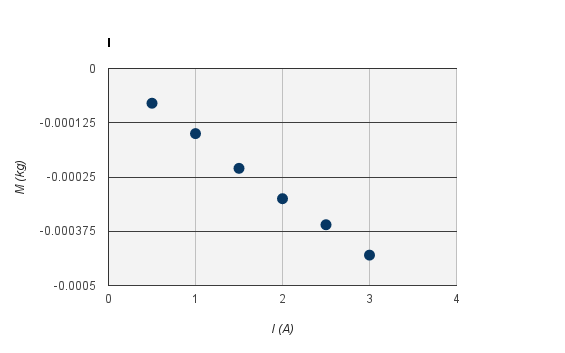
\includegraphics[width=\textwidth]{mediciones_primer_experiencia.png}
\caption{Masa en función de la corriente}
\label{fig:1}
\end{figure} 

\subsubsection{Resultados}
Se calculó la fuerza magnética restándole a las masas finales medidas el dato de la masa inicial del portaimán (Con la fuente apagada, sin corriente) y multiplicando esta diferencia por el valor de la gravedad.
\begin{equation}
F_m = (m_k - 0,1607kg)*9,98\frac{m}{s^2}
\end{equation}

\begin{table}[ht]
\centering
%%%%%%%%%%%%%%%%%%%%%%%%%%%%%%%%%%%%%%%%%%%%%%%%%%%%%%%%%%%%%%%%%%%%%%
%%                                                                  %%
%%  This is a LaTeX2e table fragment exported from Gnumeric.        %%
%%                                                                  %%
%%%%%%%%%%%%%%%%%%%%%%%%%%%%%%%%%%%%%%%%%%%%%%%%%%%%%%%%%%%%%%%%%%%%%%
\begin{tabular}{|l|c|c|r|}
\hline
I(A)	&m(kg)	&L(m)	&Fm(N)\\ \hline
0,5	&-8E-05	&0,084	&-1,60458\\
1	&-0,00015	&0,084	&-1,60528\\
1,5	&-0,00023	&0,084	&-1,60608\\
2	&-0,0003	&0,084	&-1,60678\\
2,5	&-0,00036	&0,084	&-1,60738\\
3	&-0,00043	&0,084	&-1,60808\\ \hline
\end{tabular}

\caption{Fuerza magnética en función de la corriente}
\end{table}

Con la expresión (1), obtenemos la ecuación de una recta que podemos escribir como:
\begin{equation}
F_m = I L B 
\end{equation}

Como los puntos obtenidos en las mediciones no están contenidos en una única recta, se debieron aproximar los resultados mediante cuadrados mínimos. A 
continuación se muestra el resultado aproximado:

\begin{figure}[H]
\centering
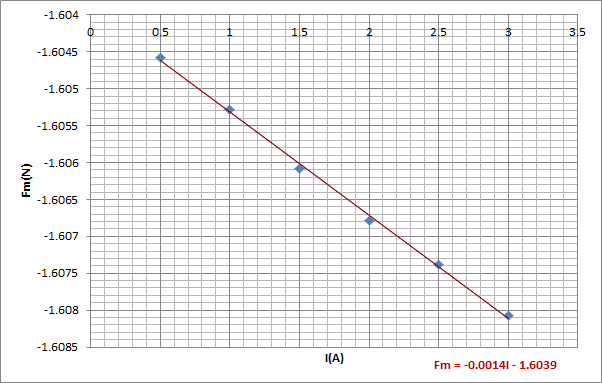
\includegraphics[width=\columnwidth]{recta_primer_experiencia}
\caption{Fuerza magnética en función de la corriente}
\end{figure}

Teniendo como recta a:
\begin{equation}
F_{m} = -0.0014 I - 1.6039
\end{equation}

Finalmente obtenemos B como:
\begin{equation}
B = \frac{pendiente}{L} = -0.017 T
\end{equation}

\subsection{Fuerza en función de la longitud del alambre}
Para esta segunda experiencia:

\begin{enumerate}
  \item Se armó el dispositivo con uno de los circuitos.
  \item Se determinó la longitud del alambre para una de las plaquetas.
  \item Se aplicó una corriente de 2A.
  \item Se determinó la "masa" del sistema.
  \item Se calculó la fuerza magnética.
  \item Se apagó la fuente, se reemplazó la plaqueta y se repitió la experiencia. 
  \item Se graficaron los resultados.
  \item Se obtuvo el campo el valor para el campo magnético B producido por el imán.
\end{enumerate}
\subsubsection{Mediciones}

Al variar la longitud del alambre en pasos se determinaron las siguientes masas para el sistema:

\begin{table}[H]
\centering
%%%%%%%%%%%%%%%%%%%%%%%%%%%%%%%%%%%%%%%%%%%%%%%%%%%%%%%%%%%%%%%%%%%%%%
%%                                                                  %%
%%  This is a LaTeX2e table fragment exported from Gnumeric.        %%
%%                                                                  %%
%%%%%%%%%%%%%%%%%%%%%%%%%%%%%%%%%%%%%%%%%%%%%%%%%%%%%%%%%%%%%%%%%%%%%%
\begin{tabular}{|c|c|}
\hline
L (m)	&M (kg)\\ \hline
0,022	&-0,00011\\
0,042	&-0,00017\\
0,032	&-0,00014\\
0,012	&-6E-05\\
0,064	&-0,00023\\
0,084	&-0,0003\\ \hline
\end{tabular}


\caption{Masa en función de la longitud}
\label{tab:segunda_experiencia}
\end{table}

y se graficaron las mediciones:

\begin{figure}[H]
\centering
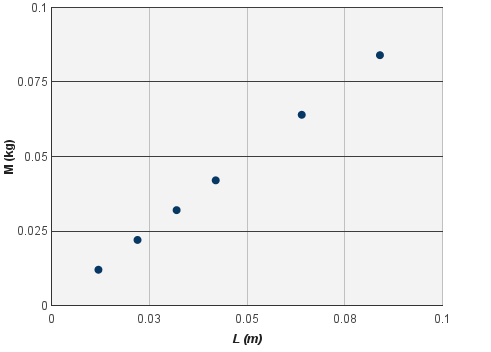
\includegraphics[width=\textwidth]{mediciones_segunda_experiencia.png}
\caption{Mediciones}
\label{fig:mediciones_segunda_experiencia}
\end{figure}

\subsubsection{Resultados}
Se calculó la fuerza magnética de la misma forma que en la primera experiencia
\begin{equation}
F_m = (m_k - 0,1607kg)*9,98\frac{m}{s^2}
\end{equation}

\begin{table}[ht]
\centering
%%%%%%%%%%%%%%%%%%%%%%%%%%%%%%%%%%%%%%%%%%%%%%%%%%%%%%%%%%%%%%%%%%%%%%
%%                                                                  %%
%%  This is a LaTeX2e table fragment exported from Gnumeric.        %%
%%                                                                  %%
%%%%%%%%%%%%%%%%%%%%%%%%%%%%%%%%%%%%%%%%%%%%%%%%%%%%%%%%%%%%%%%%%%%%%%
\begin{tabular}{|l|c|c|r|}
\hline
I(A)	&m(kg)	&L(m)	&F(N)\\ \hline
2	&-0,00011	&0,022	&-1,60488\\
2	&-0,00017	&0,042	&-1,60548\\
2	&-0,00014	&0,032	&-1,60518\\
2	&-6E-05	&0,012	&-1,60438\\
2	&-0,00023	&0,064	&-1,60608\\
2	&-0,0003	&0,084	&-1,60678\\ \hline
\end{tabular}

\caption{Fuerza magnética en función de la longitud del imán}
\end{table}

Como los puntos obtenidos en las mediciones no están contenidos en una única recta, se debieron aproximar los resultados mediante cuadrados mínimos. A 
continuación se muestra el resultado aproximado:

\begin{figure}[H]
\centering
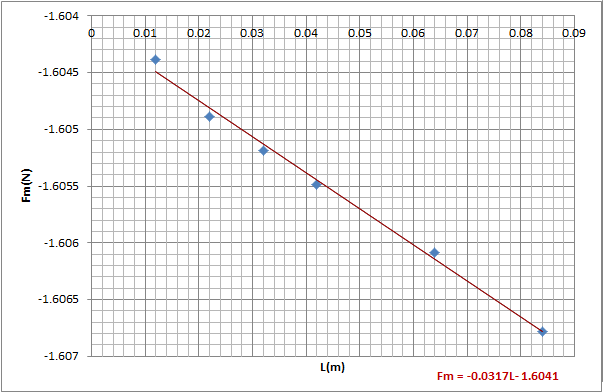
\includegraphics[width=\columnwidth]{recta_segunda_experiencia.png}
\caption{Fuerza magnética en función de la longitud del imán}
\end{figure}

Teniendo como recta a:
\begin{equation}
F_{m} = -0.0317 I - 1.6041
\end{equation}

Finalmente obtenemos B como:
\begin{equation}
B = \frac{pendiente}{I} = -0.016 T
\end{equation}

\section{Preguntas teóricas} %No supe dónde ponerlas, se vale moverlo!
1.La estadística que se hace al usar el método de cuadrados mínimos es sobre los valores absolutos de las mediciones obtenidad, sin considerar los errores que traigan los mismos. Estas incertezas, anteriormente asociadas a cada punto, se traducen en incertezas en la recta y en la ordenada al orígen de esta y se pueden calcular de la siguiente manera:


\begin{equation}
\Delta a = \Delta o \frac{n}{\sqrt{n\Sigma x_{i}^{2} - (\Sigma (x_{i})^{2} }}
\end{equation}

\begin{equation}
\Delta b = \Delta o \frac{\sqrt{\Sigma (x_{i})^{2}}}{\sqrt{n\Sigma (x_{i})^{2} - (\Sigma (x_{i}))^{2} }}
\end{equation}

\begin{equation}
\Delta o = \sqrt{\frac{1}{n-2}\Sigma(y_{i} - a x_{i} - b)^{2}}
\end{equation}


2. Es válido usar el criterio de cuadrados mínimos dado que la teoría nos manifiesta que la relación que estamos calculando es de tipo lineal.


\section{Conclusiones}

Con la realización del trabajo y el análisis de resultados, llegamos a las siguientes conclusiones:
\begin{itemize}
\item El valor final de la masa, durante la experiencia en la que variamos la corriente entre 0,5 y 3A, es aproximadamente tres veces la masa inicial.
\item Si miramos el gráfico de masa en función de la corriente, si bien no existe una recta que contenga todos los puntos, la variación de los valores tiene tendencia lineal. Por ese motivo, utilizamos cuadrados mínimos para hallar la recta.
\item La variación de la fuerza, en la primera experiencia, se observa recién en la tercer cifra decimal. La variación entre el primer y el último valor corresponde a -0,0035N.
\item Cuando se realiza la variación en la longitud del alambre y se deja fija la corriente, la masa final es entre dos y tres veces la inicial.
\item Cuando se procede a variar la longitud del alambre y mantener la corriente en 2A, la fuerza varía en -0,0019N.

\end{itemize}

\end{document}
